\documentclass[../main.tex]{subfiles}
\graphicspath{{\subfix{../images/}}}
\begin{document}
\section{Implementation}
\label{implementation}

In this section we are going to present the implementation details of this project. In particular the section is divided into five subsections that are: "Software architecture" where we present the software architecture chosen for this work, "JavaScript WebRTC Client" where we describe the front end module and the WebRTC client implementation, "Python aiortc Server" where we describe how the WebRTC server was implemented using the aiortc library, "VAD Analyzer" where we describe the implementation of the VAD part with the turn handling and status communication with web-sockets and "Dockerization" where we describe the procedure followed to make the containerization of the server.

\subsection{Software Architecture}
\label{software architecture}

As we described in the introduction of this thesis the aim of the project was to develop a real-time remote VAD. This module would be used in the Abel android to manage the turn-taking part of the robot to provide a realistic communication experience. In order to provide this realistic experience, low-latency response was the key, so all the architecture was focused on this, obviously taking into consideration also that the voice activity detection task needs to be performed with good quality. This is because we want that the robot understands well and rapidly if the turn is finished, in order to provide the response in time. So it is clear why we need a real-time VAD task. The idea for this project was to develop a remote real-time VAD in order to provide to the classification Silero VAD model enough processing power on an Abel dedicated remote server, where also all the other components of Abel runs too, for example the speech processing part. This was done to prevent that the module performance would be limited by the hardware capabilities present locally with Abel. In the Figure \ref{fig:audio workflow} is shown a high level representation of the architecture.

\begin{figure}[ht]
    \centering
    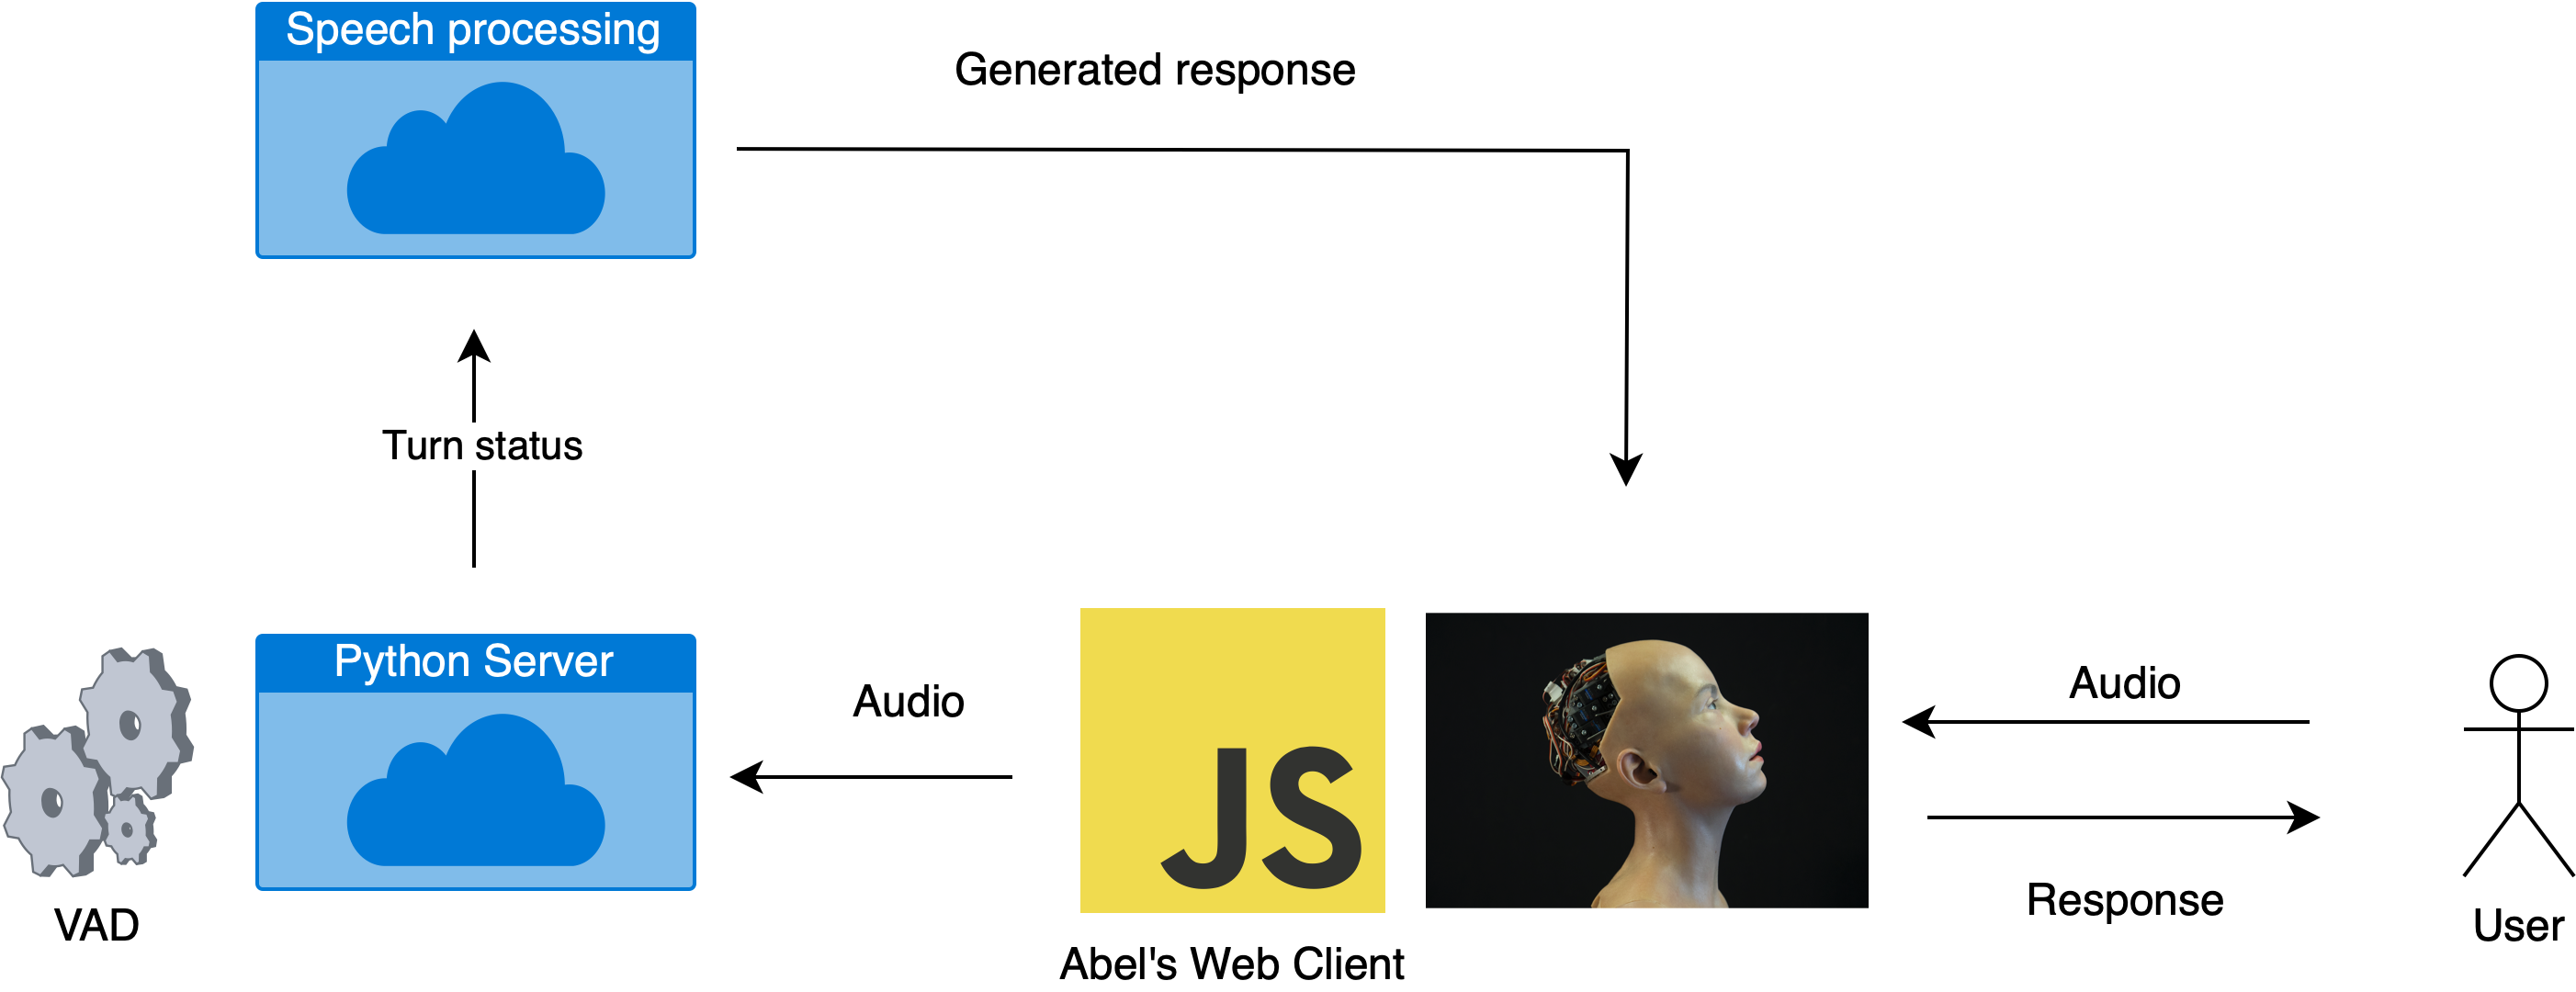
\includegraphics[width=\textwidth]{images/Audio architecture 2.png}
    \caption{Audio workflow}
    \label{fig:audio workflow}
\end{figure}

As described in section \ref{methods and methodology} in order to develop the real-time communication part of our work we used the WebRTC technology. This is a technology mainly used and developed for browsers and web applications in general. So the idea was naturally to develop a web application to transmit the audio in real time from Abel to the server. Initially we started to develop a web application that was composed of a JavaScript Client and Server, but rapidly we realized that a JavaScript Server was not a good option. This was because it lacks of support in real time processing of the audio coming from WebRTC. Furthermore that real time audio received by the JavaScript server required to be sent to the Python code that performs voice activity detection using PyTorch. This transmission of data would have increased the overall latency of the system. So in order to have an easier way to process the incoming audio from WebRTC and to reduce the latency of the system we have thought that a WebRTC Python server would be a better option. Following this consideration we decided to use the aiortc library in order to implement a WebRTC server that receives the audio and also processes it thanks to the Analyzer module. 

In the end we decided that a containerization was the correct thing to do for our turn-taking module, because of the advantages that a service-oriented architecture would produce like isolation, portability, easy dependency management and versioning. This was also a straightforward decision because all the Abel software architecture is service-oriented. 

To sum up the software architecture of this work is composed by a JavaScript Client that connects to a Python aiohttp server using WebRTC to transfer real time audio data. The Python server uses the aiortc library to receive these data. It also contains an Analyzer module that handles the turn-taking part of the application, performing the VAD task using the Silero VAD model with the PyTorch framework, and managing consequently the status of the conversation. This status is also sent to the other modules of Abel through a web-socket connection. The Python server is a containerized service using the Docker platform.

In the Figure \ref{fig:software architecture} there is a detailed representation about the software architecture of the turn-taking module developed in this work.

\begin{figure}[ht]
    \centering
    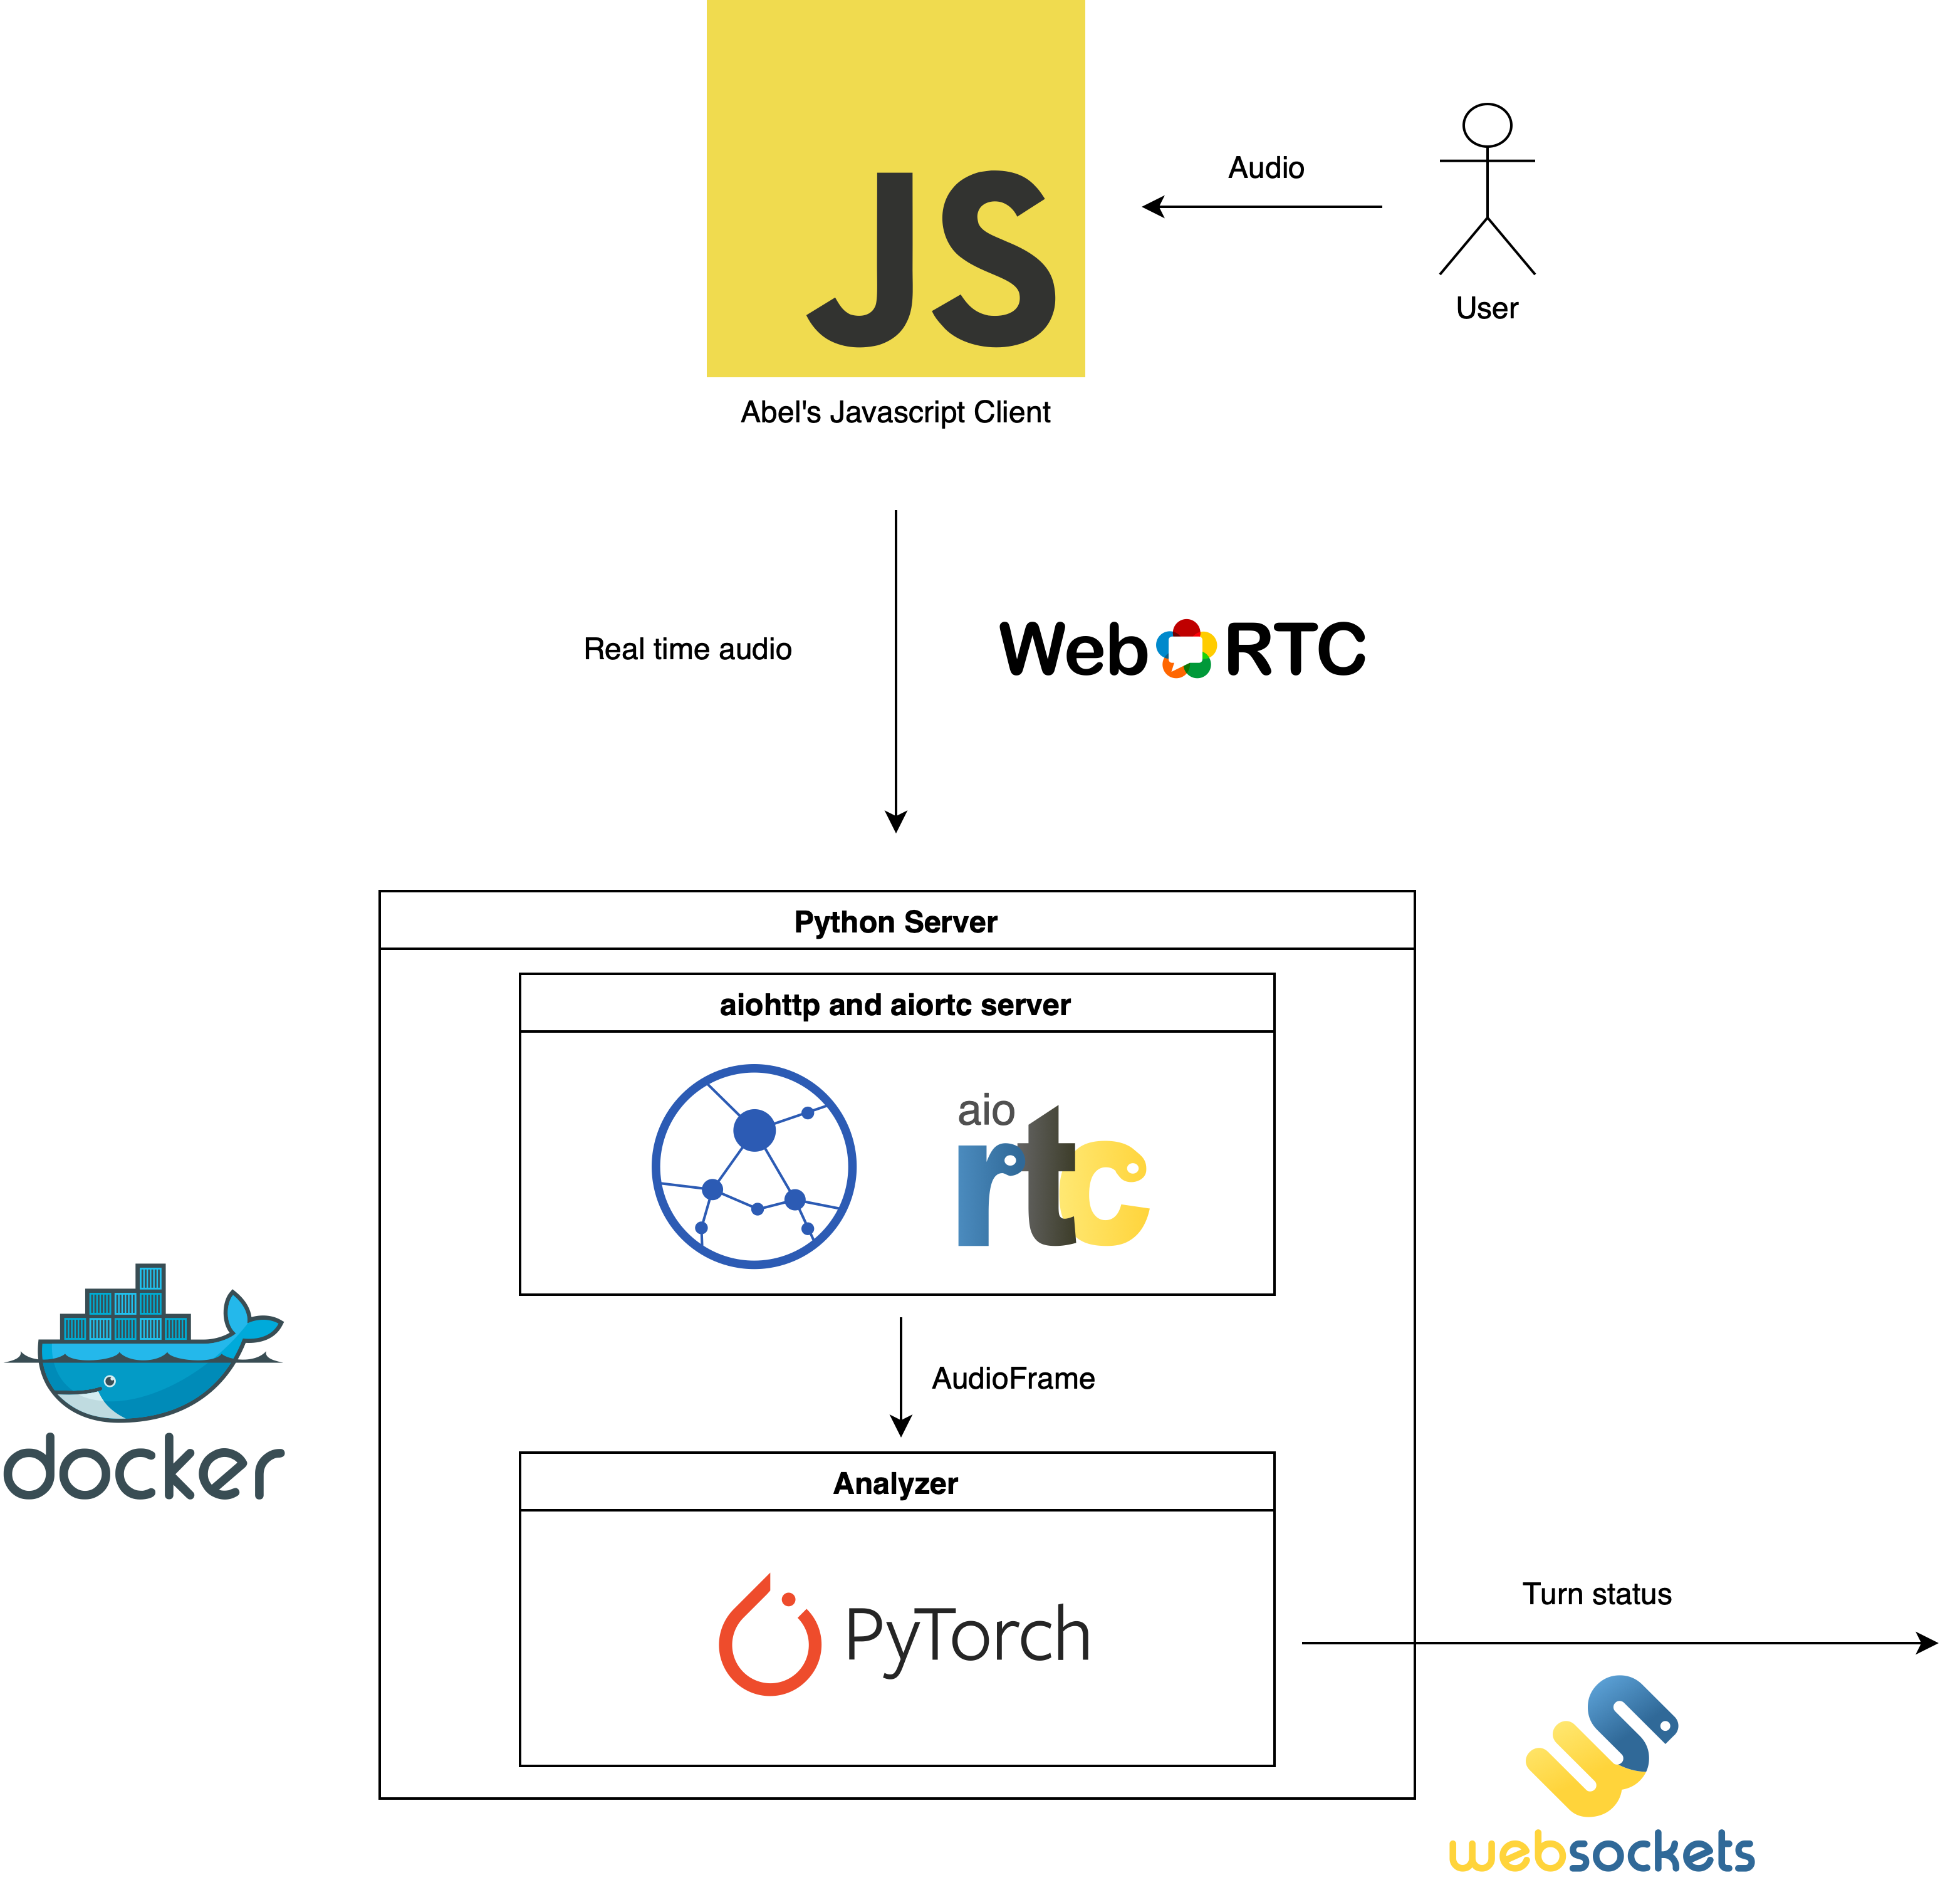
\includegraphics[width=0.95\textwidth]{images/Software architecture.png}
    \caption{Software architecture of the project}
    \label{fig:software architecture}
\end{figure}

\subsection{JavaScript WebRTC Client}

In order to perform a WebRTC connection we implemented a JavaScript Client and a Python server. The Client has the job to acquire the audio from the Abel's microphone and send it to the server establishing a WebRTC connection. In the Client is possible to select the audio source thanks to the apposite option. Then through the Start button it is possible to ask for the start of the connection and transmission of the audio. In the "Connection State" section below, it is shown the current status of the connection regarding the ICE gathering state, ICE connection state and Signaling state. To know more about these concepts please refer to the section \ref{webrtc}. Furthermore once the connection has started in the "Connection statistics" section the real time connection statistics are updated every second, showing some interesting statistics like round trip time, jitter and packets lost. In Figure \ref{fig:web interface} is shown the web application interface.

\begin{figure}[ht]
    \centering
    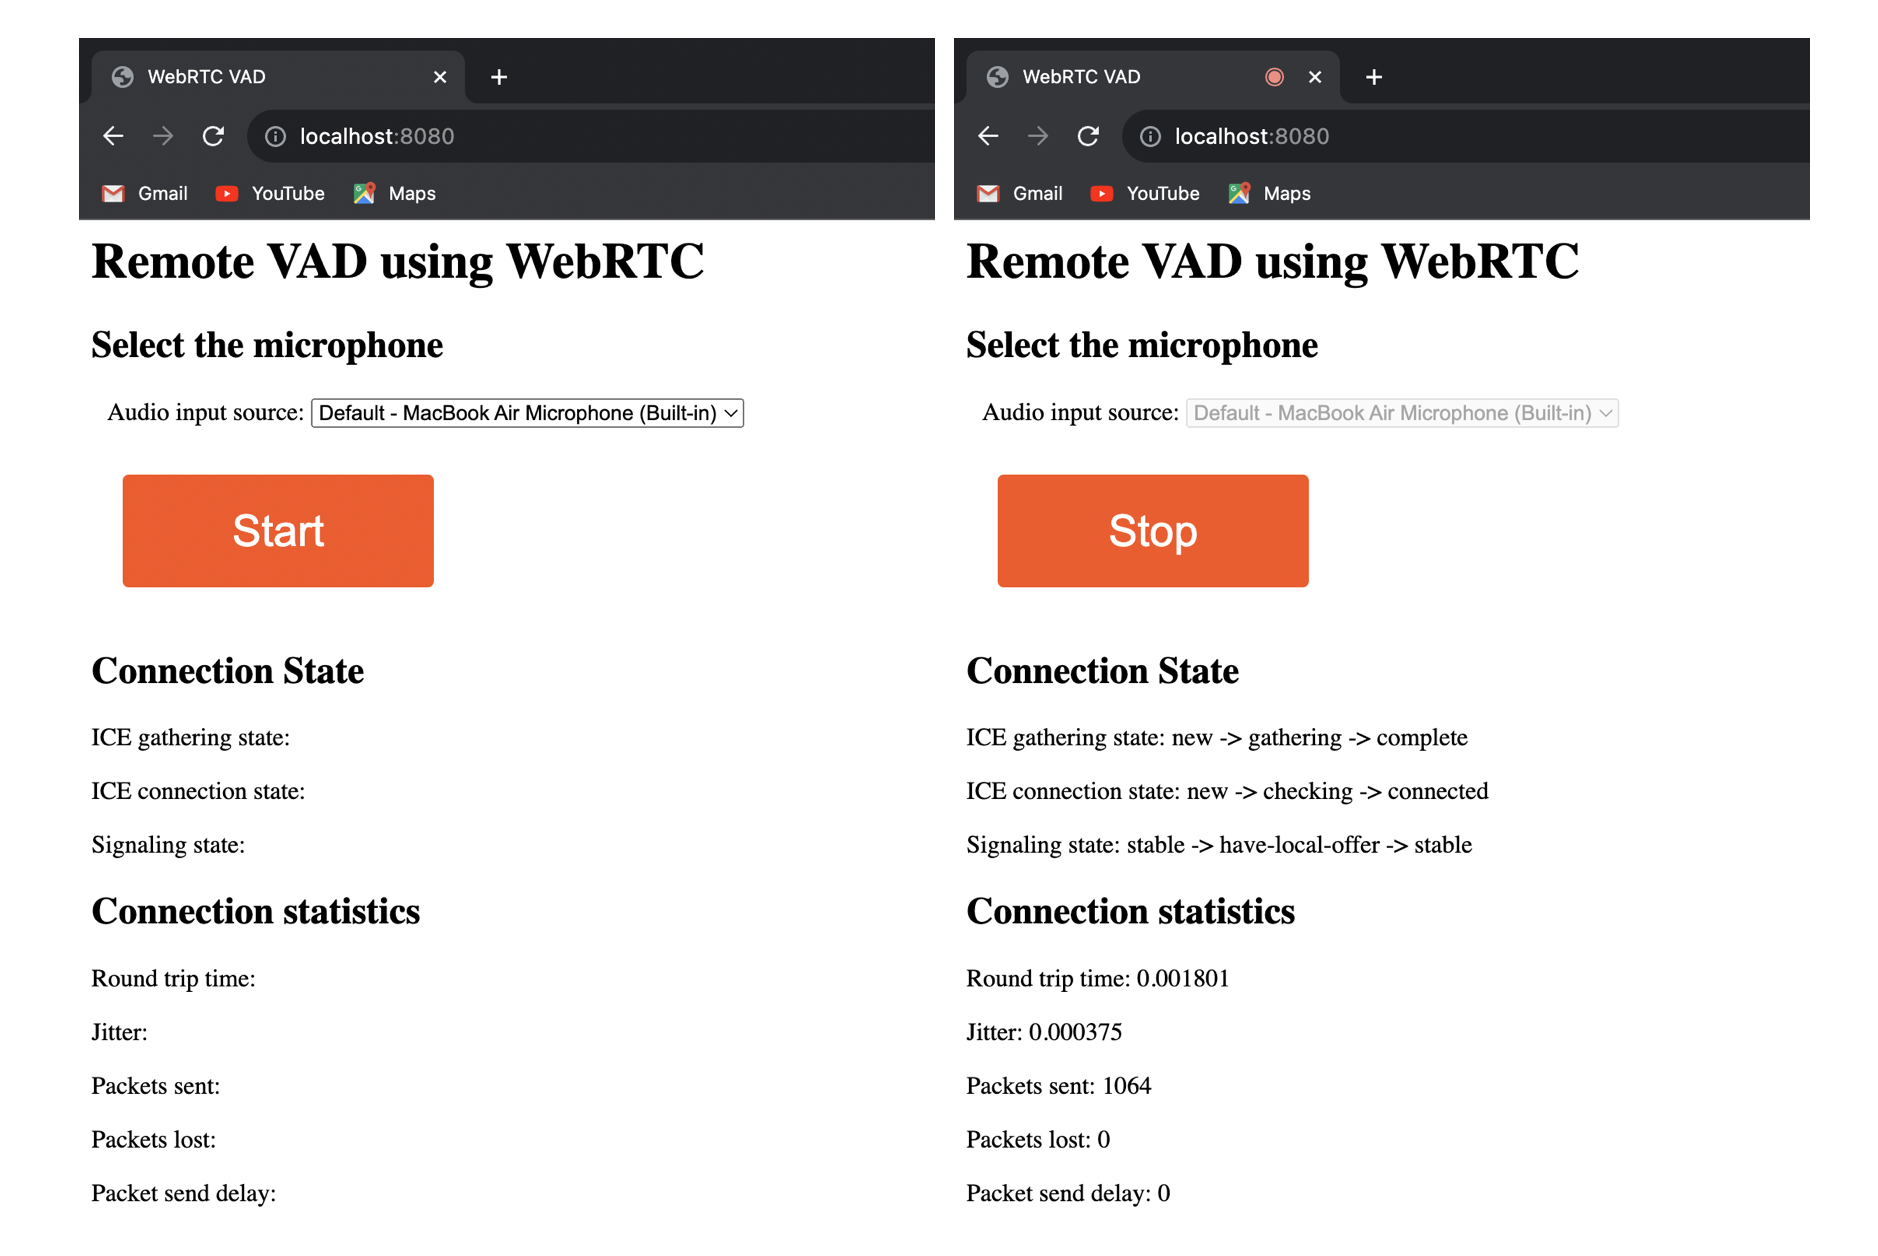
\includegraphics[width=\textwidth]{images/Web interface.png}
    \caption{Web application interface}
    \label{fig:web interface}
\end{figure}

In order to implement the option to select the audio input source for the streaming we used the \textit{navigator.mediaDevices.enumerateDevices()} method. It requests a list of the currently available media input and output devices and returns a Promise which resolves with an array of MediaDeviceInfo objects describing the devices. I than used that array to populate the selection.

The Start button calls the \textit{start()} function that initiates the procedure to create the WebRTC connection. Apart from managing the application elements, it creates the RTCPeerConnection, gets the audio stream from the microphone and adds it to the connection. Then it calls the \textit{negotiate()} function that handles the signaling part needed for the connection.  In the listing \ref{listing:pc addTrack} below is shown how the audio track is managed.

\begin{lstlisting}[language=JavaScript, caption=Audio stream handling]
//get the audio stream and adds it to the connection
navigator.mediaDevices.getUserMedia(constraints).then(function(stream){
    stream.getTracks().forEach(function (track) {
        pc.addTrack(track, stream);
    });
    return negotiate();
}, function (err) {
    alert('Could not acquire media: ' + err);
}); 
\end{lstlisting}
\label{listing:pc addTrack}

The \textit{negotiate()} function handles the signaling part of the connection. In particular here the signaling method used is an exchange of HTTP request and response. The function creates the signaling offer and waits for the completion of the ICE gathering process to complete. Then it sends the offer to the server in the body of an HTTP POST request. In the end it sets as RemoteDescription the answer received by the HTTP response. The whole procedure is realized using a chain of promises to ensure that it is done sequentially. In the listing \ref{listing:negotiate} the \textit{negotiate()} function is shown. The \textbf{pc} object shown in the code is the RTCPeerConnection object created in the \textit{createPeerConnection()} method.

\begin{lstlisting}[language=JavaScript, caption=negotiate() function implementation]
//function that create the offer and proceds with the signaling to complete the connection
function negotiate() {
    return pc.createOffer().then(function (offer) {
        return pc.setLocalDescription(offer);
    }).then(function () {
        // wait for ICE gathering to complete
        return new Promise(function (resolve) {
            if (pc.iceGatheringState === 'complete') {
                resolve();
            } else {
                function checkState() {
                    if (pc.iceGatheringState === 'complete') {
                        pc.removeEventListener('icegatheringstatechange', checkState);
                        resolve();
                    }
                }
                pc.addEventListener('icegatheringstatechange', checkState);
            }
        });
    }).then(function () {
        var offer = pc.localDescription;

        //send SDP offer to the server with http request 
        return fetch('/offer', {
            body: JSON.stringify({
                sdp: offer.sdp,
                type: offer.type
            }),
            headers: {
                'Content-Type': 'application/json'
            },
            method: 'POST'
        });
    }).then(function (response) {
        return response.json();
    }).then(function (answer) {
        return pc.setRemoteDescription(answer);
    }).catch(function (e) {
        alert(e);
    });
}
\end{lstlisting}
\label{listing:negotiate}

The Connection state update is obtained using event listeners over the events: "icegatheringstatechange", "iceconnectionstatechange" and "signalingstatechange". The obtained status is then added to the section. 

Finally, the "Connection statistics" section is updated every second showing the real time statistics of the connection. To obtain those statistics we used the \textbf{RTCPeerConnection} \textit{getStats()} method that returns a promise which resolves in a \textbf{RTCStatsReport} that contains data providing statistics about either the overall connection or about the specified \textbf{MediaStreamTrack}. In particular from the \textbf{RTCOutboundRtpStreamStats} and \textbf{RTCOutboundRtpStreamStats} we decided to show five interesting statistics \cite{statistics}:

\begin{itemize}
    \item \textbf{Round trip time}: Estimated round trip time based on the RTCP timestamps in the RTCP Receiver Report and measured in seconds. Round Trip Time (RTT) refers to the total time it takes for a data packet to travel from the source to the destination and back again.
    \item \textbf{Jitter}: Packet Jitter measured in seconds. Jitter refers to the variability in the arrival time of data packets at their destination. High jitter can lead to issues like choppy audio or video in real-time communication, as the packets may arrive too quickly or too slowly, causing disruptions in the playback.
    \item \textbf{Packets sent}: Total number of RTP packets sent. This includes retransmissions.
    \item \textbf{Packets lost}: Total number of RTP packets lost.
    \item \textbf{Packet send delay}: The total number of seconds that packets have spent buffered locally before being transmitted onto the network. The time is measured from when a packet is emitted from the RTP packetizer until it is handed over to the OS network socket.
\end{itemize}


\subsection{Python aiortc server}

The Python aiortc server has the job to receive the incoming real time audio stream from the JavaScript WebRTC client and to process the audio frames contained in the stream, passing them to the Analyzer class that will perform the VAD task. 

In order to implement a Python server we used the aiohttp library. Using this library serving a server was really easy and we used the \textit{aiohttp.web.Application()} class to create the server. Then we added the routing capabilities to it, in order to handles the http requests and we served it using the \textit{aiohttp.web.run\_app()} method. 

The asynchronous \textit{offer()} method is  of the most important of the server, since it handles the incoming signaling offer from the Client in the form of an HTTP POST request. It is called when the server receives an HTTP request at the \textit{/offer} endpoint. This method parse the offer in the payload and creates the RTCPeerConnection object. It then defines the peer connection track event handler in order to process the incoming track. Finally, it sets the received offer as remote description, creates the answer and respond to the HTTP request with it.

In order to process the incoming track, in the track event handler a relayed track is obtained from the original track thanks to the \textit{MediaRelay.subscribe()} method. It creates a proxy around the given track for a new consumer and standing to the library, this is especially useful for live tracks such as webcams or media received over the network. The relayed track is then passed to the constructor of the \textbf{AudioTrackProcessing} class together with the analyzer object created from the \textbf{Analyzer} class. This last class will be described in higher details in the next subsection.

The AudioTrackProcessing object is then added as a track, with the \textit{addTrack()} method to a media sink helper of the aiortc library that in this case is \textbf{MediaBlackHole}, since we need to consume the incoming media, but we don't need to store it, and we can discard it. If we wanted to store the incoming stream we could have used the \textbf{MediaRecorder} media sink that is a media helper from the library that writes audio and/or video to a file. In the listing \ref{listing:track event} below is shown the received track event handling in the \textit{offer()} method.

\begin{lstlisting}[language=Python, caption=Track event handling]
# prepare local media
recorder = MediaBlackhole()
analyzer = Analyzer()

# pc connectionstatechange event handler
@pc.on("connectionstatechange")
async def on_connectionstatechange():
    log_info("Connection state is %s", pc.connectionState)
    if pc.connectionState == "failed":
        await pc.close()

# pc track event handler
@pc.on("track")
def on_track(track):
    log_info("Track %s received", track.kind)

    if track.kind == "audio":
        print("Started Listening")
        relayed_audio = relay_audio.subscribe(track)  # obtain the relayed track
        # use the addTrack function to call the recv function in the AudioTrackProcessing class on the relayed track
        recorder.addTrack(AudioTrackProcessing(relayed_audio, analyzer))

    @track.on("ended")
    async def on_ended():
        log_info("Track %s ended", track.kind)
        await recorder.stop()
\end{lstlisting}
\label{listing:track event}

The \textbf{AudioTrackProcessing} class is in charge of the actual processing of the incoming track. This is because this class inherit from the \textbf{MediaStreamTrack} class that in WebRTC represents a single media track, in this case the audio, within a stream. In particular in order to "intercept" and process the incoming track we need to override the asynchronous method \textit{recv()} from the parent class. Indeed, this method is called automatically from the library when we use the incoming track. This is the reason why we needed to add the AudioTrackProcessing object to the MediaBlackHole recorder object with the \textit{addTrack()} method in the \textit{offer()} function. In this way, overriding the \textit{recv()} method every time a new track of the incoming audio is received we can process it. This is done calling the \textit{self.track.recv()} method over the track we passed in the constructor of the class. That function is a python coroutine, so we added the \textbf{await} keyword to resolve it. We could do it because we are in an asynchronous function. It is important to remember that the asynchronous call to the \textit{recv()} coroutine is done automatically by the aiortc library upon the receiving of a new track. 

The call the \textit{self.track.recv()} method returns a frame that is an \textbf{AudioFrame} of the \textbf{PyAV} python library. PyAV is a Pythonic binding for FFmpeg. The aim of the library is to provide all the power and control of the underlying library, but manage the gritty details as much as possible. PyAV allows you to perform a variety of multimedia operations, such as reading and writing audio and video files, transcoding between different formats, and manipulating multimedia streams. It also exposes a few transformations of the media data, and helps you get your data to/from other packages (e.g. Numpy and Pillow). There will be a detailed description of the tools given by PyAV to process the AudioFrame in the next subsection where the frame will actually be processed. FFmpeg instead is a comprehensive and open-source software project that provides a collection of libraries and programs for handling multimedia data. It is a powerful cross-platform solution for recording, converting, and streaming audio and video content.

The AudioFrame obtained in the \textit{recv()} method is then passed as parameter to the \textit{self.analyzer.analyze()} function that will actually manage that frame and will perform the actual processing. The analyzer is the Analyzer object that we passed in the constructor of the AudioTrackProcessing class. The class implementation is shown in the listing \ref{listing:AudioTrackProcessing} below.

\begin{lstlisting}[language=Python, caption=AudioTrackProcessing class implementation]
class AudioTrackProcessing(MediaStreamTrack):
"""
Audio stream track that processess AudioFrames from tracks.
"""

def __init__(self, track: MediaStreamTrack, analyzer: Analyzer):
    """
    Costructor of the AudioTrackProcessing class.

    Args:
        track (MediaStreamTrack): track to process
        analyzer (Analyzer): analyzer that will analyze the track
    """
    super().__init__()
    self.track = track
    self.analyzer = analyzer

async def recv(self):
    """
    Async function called from addTrack function.
    This function calls the analyze function of the analyzer passed in the constructor on the AudioFrame
    extracted from the track passed in the constructor
    """
    frame = await self.track.recv()
    self.analyzer.analyze(frame)
    return frame    
\end{lstlisting}
\label{listing:AudioTrackProcessing}

\subsection{VAD Analyzer}
\label{vad analyzer}

In this section we are going to talk about the Analyzer class. This class is implemented in the vad\_analyzer.py file, and it is instantiated by the server in the server.py file. The goal of the class is to perform the VAD task using the Silero VAD neural model, keep track of the current status of the conversation using predefined parameters and communicate this status to the other modules of the Abel android using websockets. In order to perform these activities the class depends mainly on libraries such: Pythorch, PyAV, Numpy and Websockets. First let's talk about the general idea of the work to do, and then we will move on the implementation, so to have a clearer understanding.

The idea behind this class is that when the python server receives a new connection, it instantiates a new Analyzer object that will take care of the audio streaming coming from that connection. This is why the new generated Analyzer instance is passed to the AudioTrackProcessing track in the track event handler. So the idea is that we pass the incoming AudioFrame to the Analyzer object, and it will do all the work needed. In particular, it needs to do 3 things after receiving the frame:

\begin{itemize}
    \item Preprocess the audio frame and perform the voice activity detection task over the incoming frame using the Silero VAD model inference
    \item Update the current status of the conversation, that the object keeps internally, based on the classification performed over the incoming audio and the parameters chosen 
    \item Communicate to the other modules with a websocket connection the current status of the conversation
\end{itemize}

First lets talk about the preprocessing part. The AudioFrame coming from the WebRTC connection have some feature that depends on the specific device used to acquire the audio, for example the sampling rate and the number of channels. Since the Silero model need an audio chunk with a sampling rate of 16 or 8 kHz we need to resample the incoming frame. The same is true for the number of channels, since the model require only one channel for the audio. Furthermore, we need to have control over the frame length because we want to decide the frame duration that we want to pass to the model that in any case should be longer than 30 ms. In particular the frame duration of an audio chunk depends on two factors: the number of samples contained in the frame and the sampling rate. For example a typical AudioFrame coming from WebRTC is made of 960 samples at 48 kHz with 2 channels that are a stereo layout. In this case to compute the incoming audio frame duration we need to divide the number of samples (960) by the sampling rate (48 000) obtaining a duration of 20 ms. This audio chunk duration is too short for our model, so we needed to find a way to obtain a longer frame duration with a different sampling rate in order to meet the requirements in the use of the Silero VAD model, that, just to remember, are a sampling rate of 8 or 16 kHz and, a frame duration of at least 30 ms and a mono layout (1 channel). The way we could manage our requirements was to resample the incoming frames with the desired sampling rate and to store them in a buffer in order to retrieve the correct number of samples to meet our frame duration requirements.

Once we have an audio chunk of the correct duration and the correct sampling rate we need to transform our AudioFrame in a PyTorch tensor in order to pass it to the Silero VAD model. Furthermore, for a correct evaluation of the audio chunk, the model requires that the values of the tensor are float values normalized between -1 and 1. In the Figure \ref{fig:audio preprocessing} below is shown a high level of the operations to do to preprocess the incoming audio frame.

\begin{figure}[ht]
    \centering
    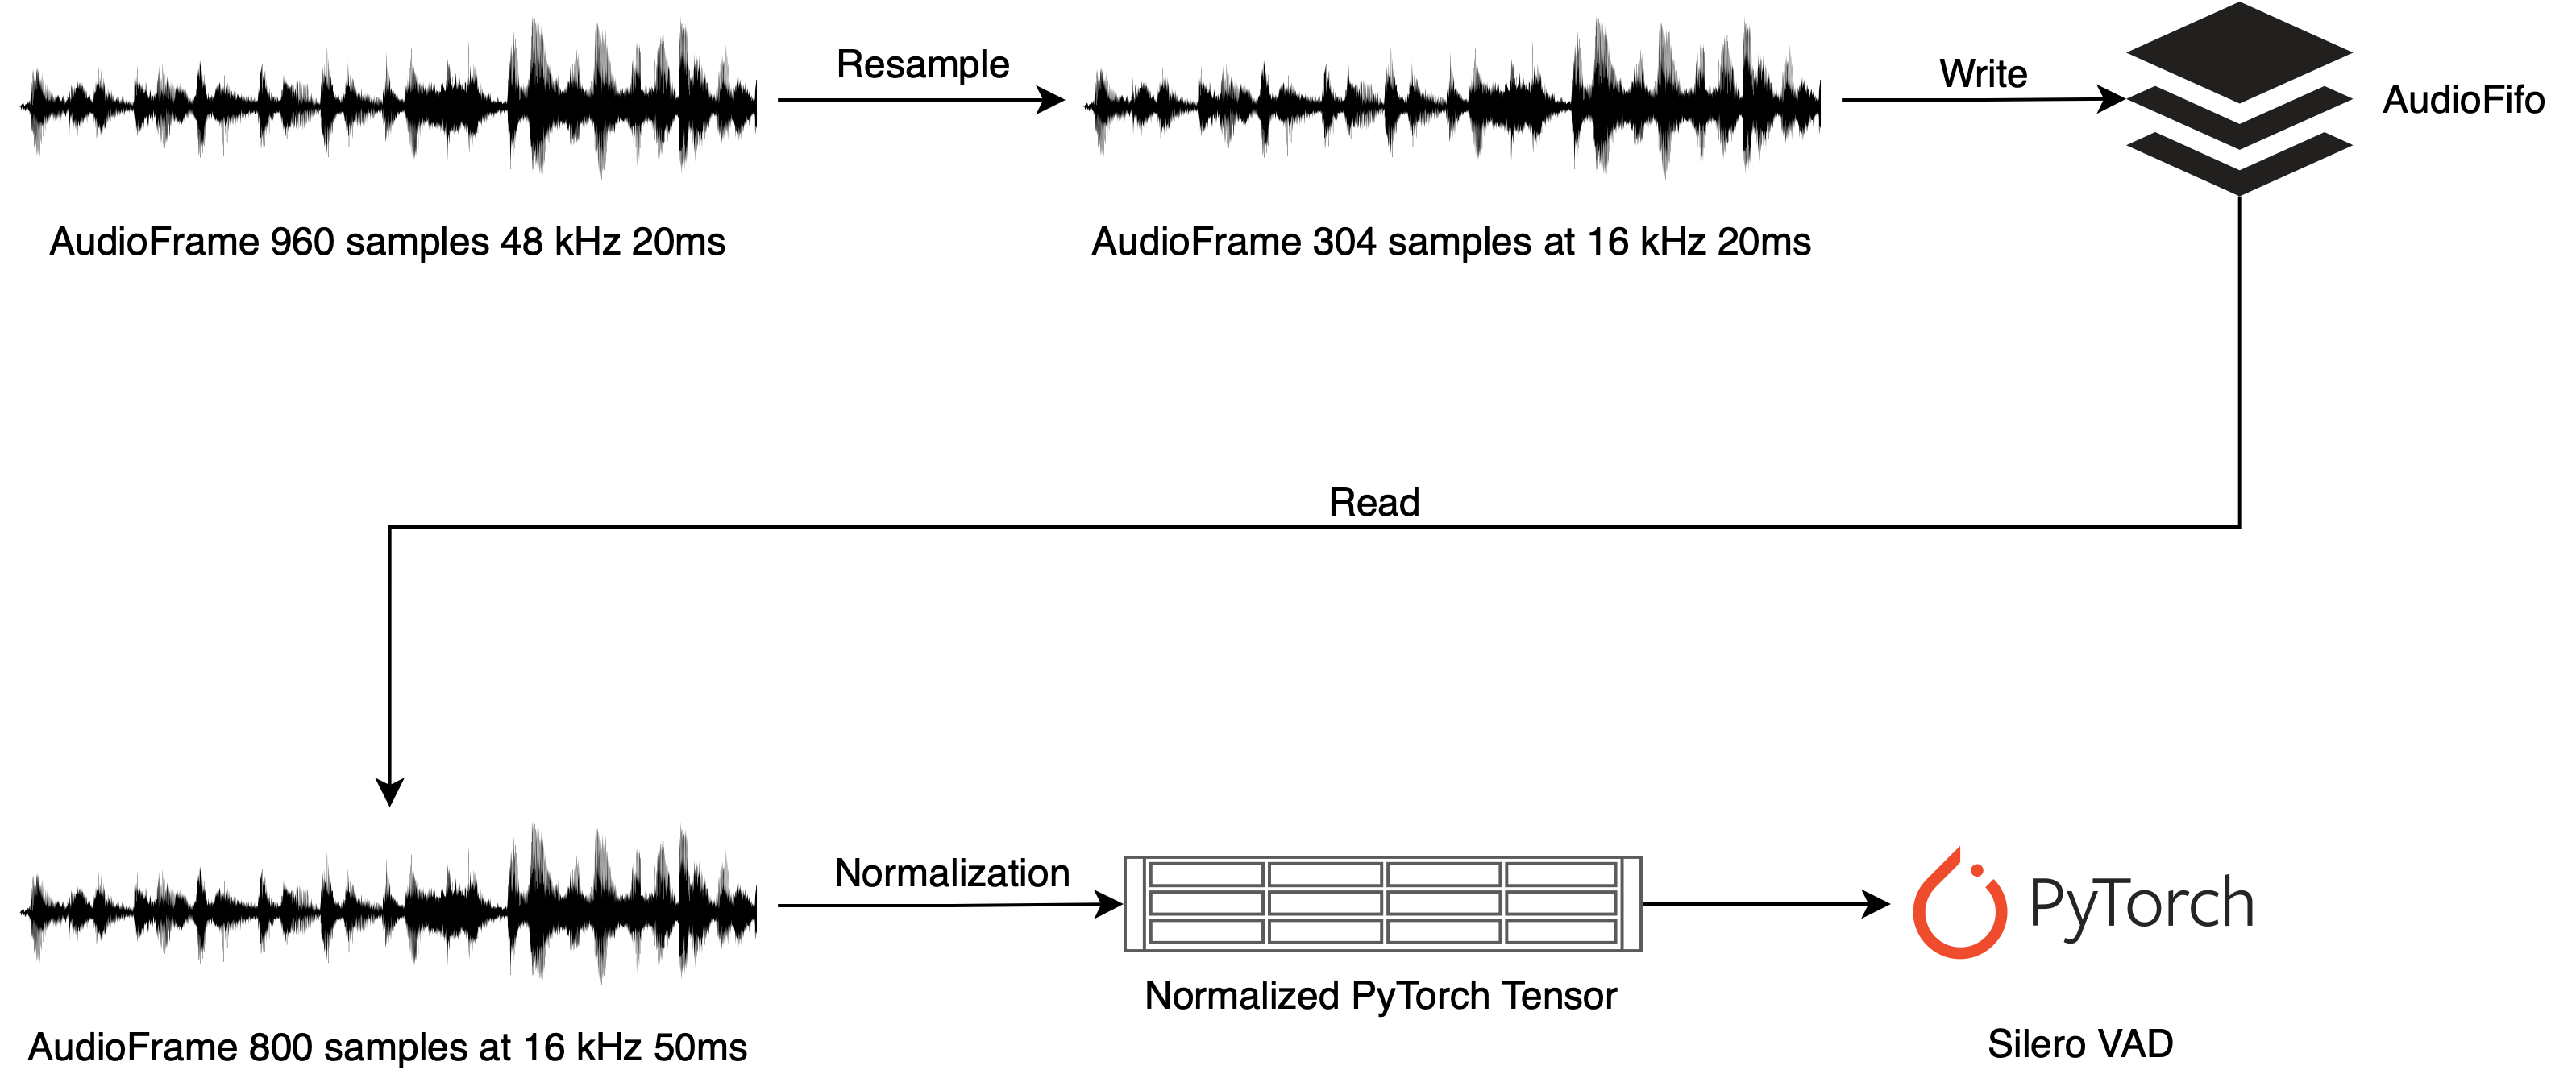
\includegraphics[width=\textwidth]{images/Audio preprocessing2.png}
    \caption{Audio preprocessing}
    \label{fig:audio preprocessing}
\end{figure}

In order to implement this preprocessing part we used two helper classes given by the PyAV library: the \textbf{AudioFifo} class and the \textbf{AudioResampler} class. The AudioFifo class is a simple audio sample FIFO (First In First Out) buffer where is possible to push a frame of samples or retrieve a determined number of samples. The AudioResampler class is a helper class able to change the format, layout and sampling rate of the incoming AudioFrame with the target parameters. 

In particular, we instantiated an AudioFifo and an AudioResampler in the constructor of the Analyzer class. The AudioResampler constructor needs three parameters that are the target parameters after the resampling operation. These parameters are: the format, that is the format in which the audio data is represented as for example the number of bytes, in the AudioFormat form; the target layout, that is the number of channels for the audio, in the AudioLayout form and the rate, that is the target sampling rate of the returning AudioFrame, in the int form. In the constructor we specified the s16 format, the "mono" layout and for the sampling rate the value found in the configuration file. 

The configuration.json file is a configuration file in the JSON format where all the parameters of the application are specified. In particular this configuration file is read in the constructor of the Analyzer class and contains both the parameters for handling the state of the conversation and other useful parameters to the Analyzer object. The parameters used in the management of the conversation will be explained in details later when we will talk about the state management while the other parameters used are:

\begin{itemize}
    \item \textbf{sampling\_rate}: it is the sampling rate passed to the Silero VAD model and consequently the target sampling rate for our audio frames after resampling 
    \item \textbf{frame\_duration}: it is the desired duration for the audio frame passed to the Silero VAD model. This duration determines how many audio samples we should take from the AudioFifo based on the target sampling rate
    \item \textbf{websocket\_port}: it is the web-socket server port to which the Analyzer will connect to communicate the current status of the conversation
\end{itemize}

When a new AudioFrame is received from the server it is passed to the \textit{analyze()} method. Here with the \textit{resample()} method the resampling part is performed. The AudioResampler.resample() method returns a list of AudioFrame with the new parameters, so we have to select the first element. Now we can write the frame to the AudioFifo with the \textit{write()} method. Then we compute the number of samples required to meet the desired audio frame duration specified in the configuration file. This is computed multiplying the desired frame duration with the target sampling rate. After we know how many samples we need, we should check if we have enough of it in the fifo buffer. The \textit{AudioFifo.read()} method requires two parameters that are the number of samples to read and a boolean specifying if it's allowed to return fewer samples than requested. Since we need the correct number of samples to meet the required frame duration we passed the value False. If in the buffer there are fewer samples than requested the method will return the value None. 

If we know that the returned AudioFrame is not None we can continue creating the PyTorch tensor for the model. First we obtain a Numpy array from our AudioFrame using the \textit{AudioFrame.to\_ndarray()} method. Second we change the type of the array from int to float 32 using the \textit{numpy.astype()} method and we normalize the values of the array between -1 and 1. In the end we use the \textit{torch.from\_numpy()} method to obtain a PyTorch tensor.

Once we have obtained our PyTorch tensor, the preprocessing part is over, and we can move to the inference part. The idea is to pass the preprocessed audio chunk to the Silero VAD model and this will return a confidence value between 0 and 1 representing the probability that the passed audio chunk actually contains speech or not. In particular, the neural model is loaded from the PyTorch Hub in the constructor of the Analyzer using the code shown in the listing \ref{listing:model load}. The loaded model is version 4.0 that is the last version released at the time of the writing of this thesis. 

\begin{lstlisting}[language=Python, caption=Silero VAD model load]
torch.set_num_threads(1)
self.vad_model, utils = torch.hub.load(
            repo_or_dir="snakers4/silero-vad",
            model="silero_vad",
            force_reload=False,
            trust_repo=True,
        )
\end{lstlisting}
\label{listing:model load}

The model is then used in the \textit{analyze()} method passing to it two parameters that are the PyTorch tensor in the correct format and the sampling rate used. The returned value is used in the \textit{set\_state()} method. This method will update the current internal state of the conversation that the Analyzer class is keeping track of, based on the results of the inference over the received audio chunk. The listing \ref{listing:analyze} below shows the \textit{analyze()} method.

\begin{lstlisting}[language=Python, caption={analyze() method}]
def analyze(self, frame):
"""
Function to analyze the input frame.

Args:
frame (AudioFrame): frame to analyze
"""
frame = self.resampler.resample(frame)[0]  # resample the audio frame with the selected sampling_rate
self.audio_fifo.write(frame)  # write the frame samples to the AudioFifo
samples = (self.frame_duration * self.sampling_rate)  # computes to samples to read needed for the specified frame duration
frame = self.audio_fifo.read(samples, False)  # reads the correct number of samples from the fifo
# if there are enough sample to analyze the desired frame duration
if frame is not None:
    # get the confidences
    tensor = torch.from_numpy(self.int2float(frame.to_ndarray())) 
    new_confidence = self.vad_model(tensor, self.sampling_rate).item()
    self.set_state(new_confidence)
\end{lstlisting}
\label{listing:analyze}

Now let's talk about how this turn-taking module handles the status of the conversation. This system uses a silence-based method since it tries to understand if the turn of the speaker is over detecting if in the audio signal there is speech or not. If the incoming audio doesn't contain speech for a certain period of time, the system will detect a turn change. As we have seen in section \ref{turn-taking} this method present one main drawback that is the handling of the pauses in the conversation. Indeed, if the speaker takes a pause longer than normal this can be mis-detected by the system as a clue for turn change even if the speaker will continue to speak normally. This would lead to a situation where the agent will start to speak overlapping to the user and creating a situation where the conversation is interrupted, and a recover mechanism should be actuated. A silence-based method typically uses a threshold to determine after how much time of silence the user finished his turn. If the pause is shorter than this threshold the system will not detect a turn change and the conversation will continue normally, while if the pause is longer than the threshold the system will detect erroneously a turn-change and will start speaking. So we can understand that this simple value is actually very critical for the performance of the system also from the point of view of the reactivity. Indeed, if the threshold value is short, for example 200 ms, the reactivity of the system will be really high because as soon as the user stops talking the system will detect the turn change and will give an answer. On the other hand this short threshold value implies that if the user takes a pause just longer than 200 ms, an easy possibility, the system will incorrectly detect a turn change. If the threshold value is too long instead, for example two seconds, the system would probably detect correctly most of the turn changes because all the user's pauses will be usually shorter than two seconds, but the system would be really slow because it will always wait at least two second after the user stops speaking to give an answer. Obviously the latency of the response from the system is given also by the time required to process the response consequently to the user's sentence. 

In order to partially alleviate the problem related to this threshold value we proposed and developed an end-of-turn detection model that is slightly more complex than a simple silence-based. The idea is to use two thresholds to detect the end of turn. The first threshold detect the potentiality of a turn change while the second threshold confirms the eventual turn change. This introduction helps the system to have a better performance in the correct detection of the end of turn and a higher reactivity. In particular the first threshold has a value that is lower than the second. When a user stops speaking and the first threshold of silence is passed the system will detect a \textbf{potential} turn change and will start to process the user sentence in order to provide the response. This response will be given only if also the second threshold of silence is respected, so this means the silence from the user is actually a turn-change. If the user starts talking again after the first threshold was passed, it means that the detected silence was a pause and the system will not speak avoiding overlapping the user. So with this system we have both the advantages of having a short threshold, because the system has a higher reactivity since the processing of the sentence of the user starts early, and of having a long threshold since the system will wait longer to be sure that the silence is not a pause but an actual turn change. In practice this is a way to partially hide the latency given by the processing of the user's sentence. 

Let's make an example to make the concept clearer. Let's start with a normal silence-based system with only one threshold. Suppose that the system processes the user's sentence in 500 ms and has a silence threshold of 700 ms. After the user stops speaking, supposing a continuous vad analysis of the audio, the system will wait 700 ms to understand if the silence is determined by a pause or by a turn change and takes 500 ms to process the audio. This means that the system in case of a turn change will reply after 1200 ms. Let's see the case with the system using 2 thresholds, one of 400 ms and the other of 700 ms, supposing a processing time of 500 ms. After the user stops talking, after 400 ms the system detects a potential turn change and starts processing the acquired audio. Now two things can happen: the user actually wants to yield the turn or the user is making a pause. If the user is making a pause and for example after 600 ms will start speaking, the system will not respond to the user and will continue to listen the sentence. If the user wants to change the turn the second threshold value of 700 ms is meet, and now we only need to wait 200 ms for the reply to come. So in the first case we waited 1200 ms for the reply, while in the second case we waited 900 ms. This happens because we started processing the sentence 300 ms earlier than the case before, but still waiting enough time to be sure that the turn is actually over. The Figure \ref{fig:new system} represents this example visually.

\begin{figure}[ht]
    \centering
    \includegraphics[width=\textwidth]{images/new system.png}
    \caption{One threshold system vs Two thresholds system}
    \label{fig:new system}
\end{figure}

The system manages the status of the conversation through a series of states that are controller by a list of thresholds that are specified in the configuration file. These values are:

\begin{itemize}
    \item \textbf{silence\_threshold}: this value indicates the first potential turn change threshold.
    \item \textbf{confirmed\_silence\_threshold}: this value indicates the second actual turn change threshold
    \item \textbf{conversation\_not\_started\_threshold}: this value indicates the time frame in which the system expects a response from the user after the end of the robot's turn
    \item \textbf{start\_conversation\_threshold}: this value indicates how much time after the user's last sentence the robot my want to start a new topic in the conversation
\end{itemize}

In particular the statuses of the conversation for the module can be:

\begin{itemize}
    \item \textbf{Not started}: the conversation is not started, and the system is waiting for a reply
    \item \textbf{Started}: the reply is started, and the system is analyzing the sentence in order to identify a turn change
    \item \textbf{Potential turn change}: the system has identified a potential turn change and is waiting to confirm the turn change in case of continued silence or will roll back in case of incoming speech
    \item \textbf{Conversation not started}: the system has detected that the user didn't respond in the predefined threshold time frame so may want to take corrective actions
\end{itemize}

Let's analyze how the status of the conversation evolves in relation to the threshold values presented before. The system starts is the state \textbf{Not started}. If silence is detected for more than the \textbf{conversation\_not\_started\_threshold} the state switch to \textbf{Conversation not started}. If silence is continued to be detected reaching the \textbf{start\_conversation\_threshold} the state come back to \textbf{Not started} and a \textit{Start conversation} message is sent to the robot's architecture. Instead if speech is detected in the \textbf{Not started} state, this is switched to \textbf{Started}. The system remains in this state until silence is detected for the \textbf{silence\_threshold}. Now the system switch to the state \textbf{Potential turn change}. In this state two things can happen: silence is detected until the \textbf{confirmed\_silence\_threshold} or speech is detected. In the first case the system detects an actual turn change and comes back to the state \textbf{Not started} in order to restart the detection phase. A \textit{Turn change confirmed} message is sent to the robot's architecture to communicate the detection of a turn change. In the second case the system realizes that the silence was cause by a pause and the state will become \textbf{Started} again. The system will send a \textit{Potential turn change aborted} so the rest of the robot's architecture knows that the processing performed is no longer required. The Figure \ref{fig:state diagram} shows the state diagram of the system.

\begin{figure}[ht]
    \centering
    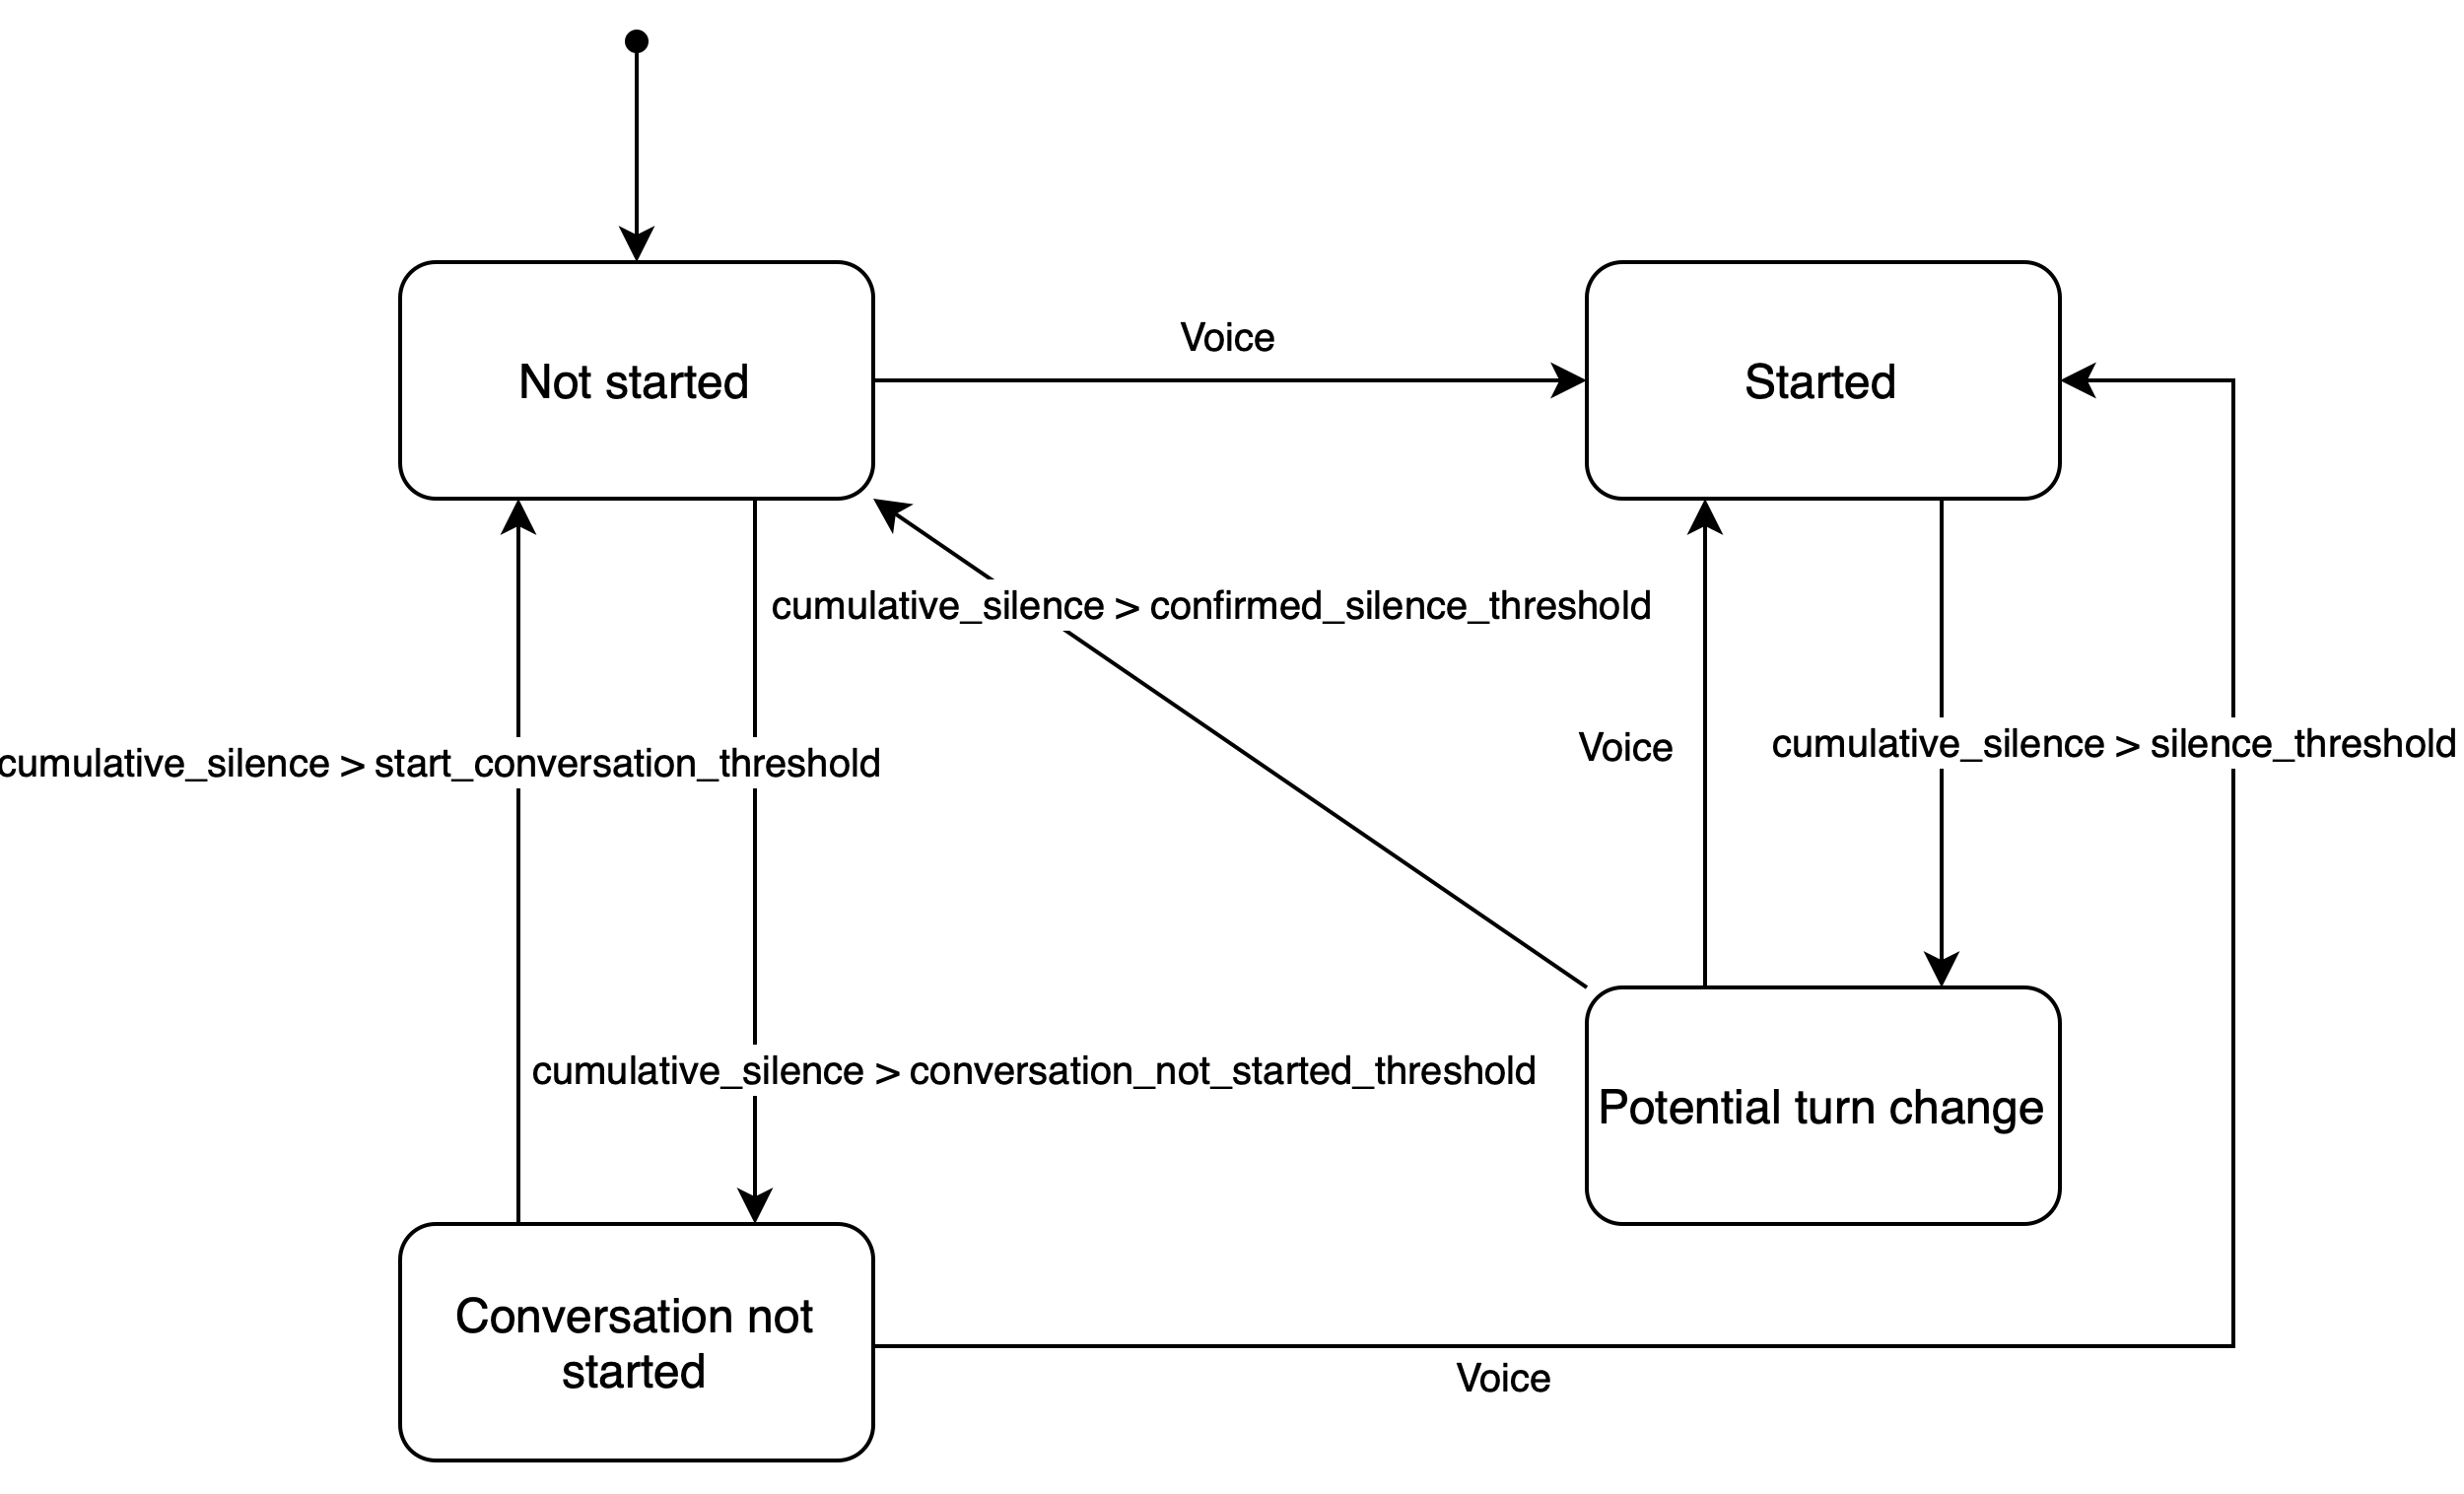
\includegraphics[width=\textwidth]{images/State diagram.png}
    \caption{State diagram}
    \label{fig:state diagram}
\end{figure}

From the implementation point of view, the status handling is straightforward. The speaking probability obtained from the inference is passed to the \textit{set\_state()} method that compares the speaking probability with the \textbf{confidence\_threshold} parameter. This parameter is defined in the configuration.json file. The comparison establishes if in the audio chunk is present speech or not. If it is not the case, the frame duration is summed up to a \textit{cumulative\_silence} parameter that keeps track of how much silence has been detected during the conversation. Subsequently, a series of if and elseif determines with the state of the system and thresholds discussed above the new state in which the system should be. In the listing \ref{listing:state} is shown the first part of the \textit{set\_state()} method to give a glance of what the method look like.

\begin{lstlisting}[language=Python, caption={set\_state() method}]
def set_state(self, speaking_probability):
"""
Function that handles the current status of the turn

Args:
speaking_probability (float): Probability detected that the input frame contains voice
"""
# check if the new frame has voice
if speaking_probability <= self.confidence_threshold:
    self.cumulative_silence += self.frame_duration
    # if there is silence for more than the specifiend threshold there could be a turn change
    if (
        self.state == Analyzer.State.STARTED
        and self.cumulative_silence >= self.silence_threshold
    ):
        self.state = Analyzer.State.POTENTIAL_TURN_CHANGE
        print("Potential turn change")
        try:
            self.websocket.send("Potential turn change")
        except error:
            print(error.errno)

    # if there is silence for more than the specified threshold there is an actual turn change
    elif (
        self.state == Analyzer.State.POTENTIAL_TURN_CHANGE
        and self.cumulative_silence >= self.confirmed_silence_threshold
    ):
        self.state = Analyzer.State.NOT_STARTED
        # we need to go back to the NOT_STARTED state to initiate a new turn
        print("Turn change confirmed")
        print(" ")
        try:
            self.websocket.send("Turn change confirmed")
        except error:
            print(error.errno)
    ...   
\end{lstlisting}
\label{listing:state}

Furthermore, in the \textit{set\_state()} method we find how the websockets connection is used to communicate the status of the conversation to the external of the turn-taking module. In particular the initial connection to the websocket server is made in the constructor of the Analyzer class to the uri specified in the \textbf{uri} parameter in the configuration file. Then with the \textit{send()} method the system sends the updated status of the conversation to the websocket server. The messages sent by the Analyzer class are:

\begin{itemize}
    \item \textbf{Potential turn change}: a potential turn change is detected, and the system is in the state \textbf{Potential turn change}.
    \item \textbf{Turn change confirmed}: the turn change detected is confirmed, and the system goes in the state \textbf{Not started}.
    \item \textbf{Conversation not started}: the system detects that the user has not started speaking and may want to repeat the last sentence.
    \item \textbf{Start conversation}: the system notice that the user has stopped interacting with the robot, so it may want to start a new conversation maybe on a new topic.
    \item \textbf{Conversation started}: the system detects speech in the incoming audio and if it was in the state \textbf{Not started} or \textbf{Conversation not started} goes to the state \textbf{Started}.
    \item \textbf{Potential turn change aborted}: the system detects speech after being in the \textbf{Potential turn change} state, so the detected silence was cause by a pause. This means that the processing of the received audio can be stopped since the user's sentence is not finished.
\end{itemize}


\subsection{Dockerization}

Dockerization refers to the process of packaging, distributing, and running applications using Docker containers. Docker is a platform that enables developers to build, package, and distribute applications in a consistent and portable way, regardless of the environment they run in. The main concepts of dockerization are:

\begin{itemize}
    \item \textbf{Containers}: Docker containers are lightweight, standalone, and executable packages that include everything needed to run a piece of software, including the code, runtime, libraries, and system tools. Containers provide consistency across different environments, from development to testing and production.
    \item \textbf{Image}: An image is a lightweight, standalone, and executable package that includes all the necessary components to run a piece of software, including the code, runtime, libraries, and system tools. Images serve as the basis for containers.
\end{itemize}

The main advantages of using docker containers are:

\begin{itemize}
    \item \textbf{Portability}: Docker containers encapsulate an application and its dependencies, making it easy to move and run the application consistently across different environments. This portability is particularly valuable for developers, as it reduces the "it works on my machine" problem.
    \item \textbf{Isolation}: Containers provide process isolation, ensuring that an application and its dependencies run in a controlled environment. This isolation makes it easier to manage dependencies and reduces conflicts between different applications running on the same host.
    \item \textbf{Resource Efficiency}: Docker containers share the host operating system's kernel, making them more lightweight compared to virtual machines. This results in improved resource utilization, enabling more efficient use of system resources.
    \item \textbf{Scalability}: Docker containers can be easily scaled up or down based on demand. This flexibility allows for efficient resource allocation and can enhance application performance during periods of high traffic.
    \item \textbf{Rapid Deployment}: Docker enables fast and consistent deployment of applications. With Docker, you can quickly spin up containers, reducing the time it takes to deploy and update applications.
    \item \textbf{Version Control and Rollback}: Docker images can be versioned, making it easy to roll back to a previous version if needed. This version control helps manage application changes and updates effectively.
\end{itemize}

In particular to create the image of the server we created a Dockerfile. This is almost a standard file where we modified only two things. First, differently from the template file we created a home directory for the user that will launch the server. This is because we need to download the Silero VAD model from PyTorch hub and this is usually done in the home of the user. Second, we added the command "RUN apt-get -y install libgomp1". This is because this Ubuntu package is needed by the Torchaudio library. Furthermore, the server needs to expose the port to reach it. This is done running the container with the option "-p 127.0.0.1:8080:8080". This option link the port 8080 of the host with the port 8080 of the container, so we can reach the container port through the host's port.

\end{document}
